\documentclass[12pt,a4paper]{article}
\usepackage{ctex}
\usepackage{amsmath,amscd,amsbsy,amssymb,latexsym,url,bm,amsthm}
\usepackage{epsfig,graphicx,subfigure}
\usepackage{enumitem,balance}
\usepackage{wrapfig}
\usepackage{mathrsfs,euscript}
\usepackage[usenames]{xcolor}
\usepackage{hyperref}
\usepackage[vlined,ruled,linesnumbered]{algorithm2e}
\usepackage{array}
\hypersetup{colorlinks=true,linkcolor=black}

\graphicspath{{/Users/weifutao/Desktop/Algorithm_and_Complexity/Labs/Lab6-LinearProgramming}}
\newtheorem{theorem}{Theorem}
\newtheorem{lemma}[theorem]{Lemma}
\newtheorem{proposition}[theorem]{Proposition}
\newtheorem{corollary}[theorem]{Corollary}
\newtheorem{exercise}{Exercise}
\newtheorem*{solution}{Solution}
\newtheorem{definition}{Definition}
\theoremstyle{definition}

\renewcommand{\thefootnote}{\fnsymbol{footnote}}

\newcommand{\postscript}[2]
 {\setlength{\epsfxsize}{#2\hsize}
  \centerline{\epsfbox{#1}}}

\renewcommand{\baselinestretch}{1.0}

\setlength{\oddsidemargin}{-0.365in}
\setlength{\evensidemargin}{-0.365in}
\setlength{\topmargin}{-0.3in}
\setlength{\headheight}{0in}
\setlength{\headsep}{0in}
\setlength{\textheight}{10.1in}
\setlength{\textwidth}{7in}
\makeatletter \renewenvironment{proof}[1][Proof] {\par\pushQED{\qed}\normalfont\topsep6\p@\@plus6\p@\relax\trivlist\item[\hskip\labelsep\bfseries#1\@addpunct{.}]\ignorespaces}{\popQED\endtrivlist\@endpefalse} \makeatother
\makeatletter
\renewenvironment{solution}[1][Solution] {\par\pushQED{\qed}\normalfont\topsep6\p@\@plus6\p@\relax\trivlist\item[\hskip\labelsep\bfseries#1\@addpunct{.}]\ignorespaces}{\popQED\endtrivlist\@endpefalse} \makeatother

\begin{document}
\noindent

%========================================================================
\noindent\framebox[\linewidth]{\shortstack[c]{
\Large{\textbf{Lab06-Linear Programming}}\vspace{1mm}\\
CS214-Algorithm and Complexity, Xiaofeng Gao, Spring 2020.}}
\begin{center}
\footnotesize{\color{red}$*$ If there is any problem, please contact TA Yiming Liu. }

\footnotesize{\color{blue}$*$ Name: Futao Wei  \quad Student ID: 518021910750 \quad Email: weifutao@sjtu.edu.cn}
\end{center}
\begin{enumerate}

   \item 
   \textbf{Controlling Air Pollution. }The three main types of pollutants in an airshed are particulate matter, sulfur oxides, and hydrocarbons. The new standards require that the steelworks reduce its annual emission of these pollutants by the amounts shown in the following table: 
	\begin{table}[h]
		\footnotesize
		\centering
	    \label{standards}
	    \renewcommand\arraystretch{1.1}
		\begin{tabular}{lc}
			
			\hline
			\textbf{Pollutant} & \textbf{\begin{tabular}[c]{@{}c@{}}Required Reduction in Annual \\ Emission Rate (Million Pounds)\end{tabular}} \\ \hline
			Particulates       & 60                                                                                                              \\
			Sulfur oxides      & 150                                                                                                             \\
			Hydrocarbons       & 125                                                                                                             \\ \hline
		\end{tabular}
	\end{table}
    \par The steelworks has two primary sources of pollution, namely, the blast furnaces for making pig iron and the open-hearth furnaces for changing iron into steel. In both cases the engineers have decided that the most effective types of abatement methods are (1) increasing the height of the smokestacks, (2) using filter devices (including gas traps) in the smokestacks, and (3) including cleaner, high-grade materials among the fuels for the furnaces. Note that each of these methods has a technological limit on how heavily it can be used (e.g., a maximum feasible increase in the height of the smokestacks), but there also is considerable
    flexibility for using the method at a fraction of its technological limit.
    \par The following table shows how much emission (in millions of pounds per year) can be eliminated from each type of furnace by fully using any abatement method to its technological limit. For purposes of analysis, it is assumed that each method also can be used less fully to achieve any fraction of the emission-rate reductions shown in this table. Furthermore, the fractions can be different for blast furnaces and for open-hearth furnaces. For either type of furnace, the emission reduction achieved by each method is not substantially affected by whether the other methods also are used.  
    \begin{table}[h]
 	\footnotesize
 	\centering
 	\label{reduction}
 	\renewcommand\arraystretch{1.1}
 	\begin{tabular}{ccccccc}
 		\hline
 		\textbf{}          & \multicolumn{2}{c}{\textbf{Taller Smokestacks}}                                                                                           & \multicolumn{2}{c}{\textbf{Filters}}                                                                                                       & \multicolumn{2}{c}{\textbf{Better Fuels}}                                                                                                   \\ \hline
 		\textbf{Pollutant} & \textbf{\begin{tabular}[c]{@{}c@{}}Blast\\ Furnaces\end{tabular}} & \textbf{\begin{tabular}[c]{@{}c@{}}Open-Hearth\\ Furnaces\end{tabular}} & \textbf{\begin{tabular}[c]{@{}c@{}}Blast\\ Furnaces\end{tabular}} & \textbf{\begin{tabular}[c]{@{}c@{}}Open-Hearth\\ Furnaces\end{tabular}} & \textbf{\begin{tabular}[c]{@{}c@{}}Blast\\ Furnaces\end{tabular}} & \textbf{\begin{tabular}[c]{@{}c@{}}Open-Hearth\\ Furnaces\end{tabular}} \\ \hline
 		Particulates       & 12  & 9   & 25 & 20 & 17 & 13                                                   \\
 		Sulfur oxides      & 35 & 42  & 18  & 31  & 56 & 49\\                                                                      
 		Hydrocarbons       & 37  & 53  & 28  & 24  & 29  & 20\\                                                                       \hline
 	\end{tabular}
 \end{table}

    The total annual cost from the maximum feasible use of an abatement method  (in millions of dollars) was shown in the following table.  The board of directors wants to figure out how to achieve these reductions with minimum annual cost. Please design a scheme for them.
   
    \begin{table}[h]
    	\centering
    	\footnotesize
    	\label{annualcost}
        \renewcommand\arraystretch{1.1}
    	\begin{tabular}{lclcl}
    		\hline
    		\multicolumn{1}{c}{\textbf{Abatement Method}} & \multicolumn{2}{c}{\textbf{Blast Furnaces}} & \multicolumn{2}{c}{\textbf{Open-Health Furnaces}} \\ \hline
    		Taller smokestacks                             & \multicolumn{2}{c}{8}                       & \multicolumn{2}{c}{10}                           \\
    		Filters                                        & \multicolumn{2}{c}{7}                       & \multicolumn{2}{c}{6}                            \\
    		Better fuels                                   & \multicolumn{2}{c}{11}                      & \multicolumn{2}{c}{9}                            \\ \hline
    	\end{tabular}
        
    \end{table}
     
    
    \begin{enumerate}
    	\item Formulate a linear programming with necessary explanations.
    	\item
    	Transform your LP into its standard form.
    	\item
    	Transform your LP into its dual form.
    	\item 
    	Assume that the clean air standards have been relaxed. The steelworks only needs to meet any two of the three pollutants emission standards. Please update your LP in (a) to satisfy the relaxed clean air standards. {\color{blue}(Hint: You can refer to Reference14-ModelFormulation.pdf)}
    	
    \end{enumerate}
     
    \begin{solution}
    	\hfill
    	\begin{enumerate}
    		\item 
    		Suppose we make use of the $6$ abatement methods by a fraction of $x_i$, $i = 1, 2, \cdots , 6$, respectively. Hence $0 \leq x_i \leq 1$, $i = 1, 2, \cdots , 6$. \\
    		We aim to minimize the annual cost, i.e., $8x_1 + 10x_2 + 7x_3 + 6x_4 + 11x_5 + 9x_6$, while meeting the reduction goals: 
    		\begin{align*}
	    		12x_1 + 9x_2 + 25x_3 + 20x_4 + 17x_5 + 13x_6 & \geq 60 \\
	    		35x_1 + 42x_2 + 18x_3 + 31x_4 + 56x_5 + 49x_6 & \geq 150 \\
	    		37x_1 + 53x_2 + 28x_3 + 24x_4 + 29x_5 + 20x_6 & \geq 125
    		\end{align*}
    		In summary, we have the LP formulation below: 
    		\[\text{min } f(x_1, x_2, \cdots , x_6) = 8x_1 + 10x_2 + 7x_3 + 6x_4 + 11x_5 + 9x_6\]
    		\begin{align*}
	    		s.t. \quad 12x_1 + 9x_2 + 25x_3 + 20x_4 + 17x_5 + 13x_6 & \geq 60 \\
	    		35x_1 + 42x_2 + 18x_3 + 31x_4 + 56x_5 + 49x_6 & \geq 150 \\
	    		37x_1 + 53x_2 + 28x_3 + 24x_4 + 29x_5 + 20x_6 & \geq 125 
    		\end{align*}
    		\[0 \leq x_i \leq 1, \, i = 1, 2, \cdots , 6\]
    		\item
    		\[\text{max } -8x_1 - 10x_2 - 7x_3 - 6x_4 - 11x_5 - 9x_6\]
    		\begin{align*}
    		s.t. \quad -12x_1 - 9x_2 - 25x_3 - 20x_4 - 17x_5 - 13x_6 & \leq -60 \\
    		-35x_1 - 42x_2 - 18x_3 - 31x_4 - 56x_5 - 49x_6 & \leq -150 \\
    		-37x_1 - 53x_2 - 28x_3 - 24x_4 - 29x_5 - 20x_6 & \leq -125 \\
    		x_i & \leq 1 , \, i = 1, 2, \cdots , 6
    		\end{align*}
    		\[x_i \geq 0 , \, i = 1, 2, \cdots , 6\]
    		
    		\item
    		\[\text{min } -60y_1 - 150y_2 - 125y_3 + y_4 + y_5 + y_6 + y_7 + y_8 + y_9\]
    		\begin{align*}
	    		s.t. \quad -12y_1 - 35y_2 - 37y_3 + y_4 & \geq -8 \\
	    		-9y_1 - 42y_2 - 53y_3 + y_5 & \geq -10 \\
	    		-25y_1 - 18y_2 - 28y_3 + y_6 & \geq -7 \\
	    		-20y_1 - 31y_2 - 24y_3 + y_7 & \geq -6 \\
	    		-17y_1 - 56y_2 - 29y_3 + y_8 & \geq -11 \\
	    		-13y_1 - 49y_2 - 20y_3 + y_9 & \geq -9 	    		
    		\end{align*}
    		\[y_i \geq 0 , \, i = 1,2, \cdots , 9\]
    		
    		\item
    		\[\text{max } -8x_1 - 10x_2 - 7x_3 - 6x_4 - 11x_5 - 9x_6\]
    		\begin{align*}
    		s.t. \quad -12x_1 - 9x_2 - 25x_3 - 20x_4 - 17x_5 - 13x_6 & \leq -60 + M y_1 \\
    		-35x_1 - 42x_2 - 18x_3 - 31x_4 - 56x_5 - 49x_6 & \leq -150 + M y_2 \\
    		-37x_1 - 53x_2 - 28x_3 - 24x_4 - 29x_5 - 20x_6 & \leq -125 + M y_3 \\
    		x_i & \leq 1 , \, i = 1, 2, \cdots , 6
    		\end{align*}
    		\[y_1 + y_2 + y_3 = 1\]
    		\[y_i \text{ is binary } , i = 1,2,3\]
    		\[x_i \geq 0 , \, i = 1, 2, \cdots , 6\]
    		where $M$ is an extremely large positive number, say, $200$. 
    	\end{enumerate}
    \end{solution}
    
	\item 
	\textbf{Factory Production. }An engineering factory makes seven products (PROD 1 to PROD 7) on the following machines: four grinders, two vertical drills, three horizontal drills, one borer and two planer. Each product yields a certain contribution to profit (in \pounds/unit). These quantities (in \pounds/unit) together with the unit production times (hours) required on each process are given below. A dash indicates that a product does not require a process.
	
	\begin{table}[htbp]
		\scriptsize
		\centering
		\renewcommand\arraystretch{1.1}
		\begin{tabular}{m{0.18\textwidth} m{0.07\textwidth}<{\centering} m{0.07\textwidth}<{\centering} m{0.07\textwidth}<{\centering} m{0.07\textwidth}<{\centering} m{0.07\textwidth}<{\centering} m{0.07\textwidth}<{\centering} m{0.07\textwidth}<{\centering}}
			\hline
			& \textbf{PROD 1} & \textbf{PROD 2} & \textbf{PROD 3} & \textbf{PROD 4} & \textbf{PROD 5} & \textbf{PROD 6} &  \textbf{PROD 7} \\\hline
			Contribution to profit & 10 & 6 & 8 & 4 & 11 & 9 & 3 \\
			Grinding & 0.5 & 0.7 & 0.2 & - & 0.3 & 0.2 & 0.5 \\
			Vertical drilling & 0.1 & 0.2 & 0 & 0.3 & - & 0.6 & - \\
			Horizontal drilling & 0.2 & - & 0.8 & - & - & - & 0.6 \\
			Boring & 0.05 & 0.03 & - & 0.07 & 0.1 & - & 0.08 \\
			Planing & - & - & 0.01 & - & 0.05 & 0.02 & 0.04 \\
			\hline
		\end{tabular}
	\end{table}
	
	There are marketing limitations on each product in each month, given in the following table:
	
	\begin{table}[htbp]
		\scriptsize
		\centering
		\renewcommand\arraystretch{1.1}
		\begin{tabular}{m{0.1\textwidth} m{0.07\textwidth}<{\centering} m{0.07\textwidth}<{\centering} m{0.07\textwidth}<{\centering} m{0.07\textwidth}<{\centering} m{0.07\textwidth}<{\centering} m{0.07\textwidth}<{\centering} m{0.07\textwidth}<{\centering}}
			\hline
			& \textbf{PROD 1} & \textbf{PROD 2} & \textbf{PROD 3} & \textbf{PROD 4} & \textbf{PROD 5} & \textbf{PROD 6} &  \textbf{PROD 7} \\\hline
			January & 500 & 1000 & 300 & 300 & 800 & 200 & 100 \\
			February & 600 & 500 & 200 & 0 & 400 & 300 & 150 \\
			March & 300 & 600 & 0 & 0 & 500 & 400 & 100 \\
			April & 200 & 300 & 400 & 500 & 200 & 0 & 100 \\
			May & 0 & 100 & 500 & 100 & 1000 & 300 & 0 \\
			June & 500 & 500 & 100 & 300 & 1100 & 500 & 60 \\
			\hline
		\end{tabular}
	\end{table}
	
	It is possible to store up to 100 of each product at a time at a cost of \pounds0.5 per unit per month (charged at the end of each month according to the amount held at that time). There are no stocks at present, but it is desired to have a stock of exactly 50 of each type of product at the end of June. The factory works six days a week with two shifts of 8h each day. It may be assumed that each month consists of only 24 working days. Each machine must be down for maintenance in one month of the six. No sequencing problems need to be considered.
	
	When and what should the factory make in order to maximize the total net profit?
	
	\begin{enumerate}
		\item
		Use \emph{CPLEX Optimization Studio} to solve this problem. Describe your model in \emph{Optimization Programming Language} (OPL). Remember to use a separate data file (.dat) rather than embedding the data into the model file (.mod).
		
		\item
		Solve your model and give the following results.
		\begin{enumerate}
			\item
			For each machine:
			\begin{enumerate}
				\item
				the month for maintenance.
			\end{enumerate}
			\item
			For each product:
			\begin{enumerate}
				\item
				The amount to make in each month.
				\item
				The amount to sell in each month.
				\item
				The amount to hold at the end of each month.
			\end{enumerate}
			\item
			The total selling profit.
			\item
			The total holding cost.
			\item
			The total net profit (selling profit minus holding cost).
		\end{enumerate}
	\end{enumerate}
	\begin{solution}
		The month for maintenance for each machine is $2455, 25, 566, 4, 56$ for grinders, vertical drills, horizontal drills, borers, and planers, respectively. \\
		The amount to make in each month for each product (rows for product types, columns for months, same below): \\
		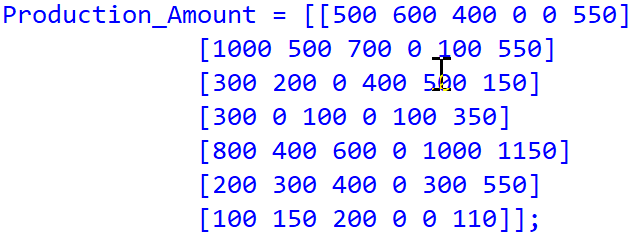
\includegraphics[scale=0.9]{production.png} \\
		The amount to sell in each month for each product: \\
		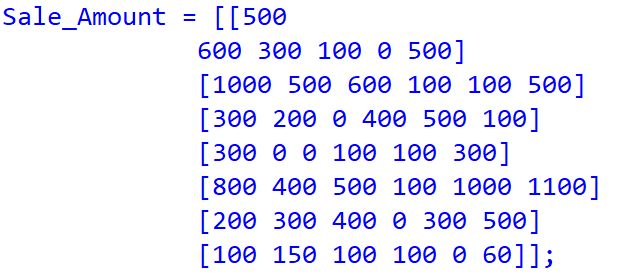
\includegraphics[scale=0.9]{sale.png} \\
		The amount to hold in each month for each product: \\
		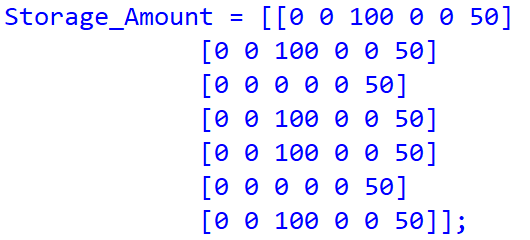
\includegraphics[scale=0.9]{storage.png} \\
		The total selling profit is \pounds 111730. \\
		The total holding cost is \pounds 425. \\
		The total net profit is \pounds 111305. 
	\end{solution}
\end{enumerate}



\textbf{Remark:} Include your .pdf, .tex, .oplproject, .project, .mod and .dat files for uploading.


%========================================================================
\end{document}
